\documentclass[a4paper,12pt]{article}
\usepackage{setspace}
\usepackage{amsmath}
\usepackage{algorithm}
\usepackage{algorithmic}
\usepackage{graphicx}
\usepackage{subfigure}
\usepackage{hyperref}
\usepackage{indentfirst}
\hypersetup{
	colorlinks=true,
	linkcolor=blue,
	filecolor=cyan,
	urlcolor=red,
	citecolor=green,
}
\author{Li Miao\\miao0044}
\title{Study of the travelling salesperson problem}
\date{\today}

\begin{document}
\onehalfspacing
\maketitle

\section{Introduction}

	 In this report, I will apply simulated annealing (SA) and genetic algorithm (GA) to travelling salesperson problem (TSP). TSP is a typical NP-hard problem, and hence many stochastic optimization algorithms have been proposed to solve it. Among the algorithms, SA and GA are the most popular and simple two. This report will discuss the implementation detail and performance.

\section{Literature Review}

	\subsection{Travelling Salesperson Problem}
	The travelling salesperson problem (TSP) says that, a salesperson, who makes a round trip visiting all the other cities  and return home, wants to minimize the total distance. Note that each city must be visited only one time. Also we assume that the distance of each pair of cities is the shortest distance, i.e., the Euclidean distance, between them. TSP regards with many real applications in reality including distributing problem \cite{ref1}. Hence, it is an important problem in operation research and computer science. However, it is a typical NP-hard problem, which cannot be solved in polynomial time.

	 From a broader view, TSP is a kind of `combinatorial optimization' problems \cite{ref2}, in which a discrete set of choices result in a pay-off which is to be maximized or a cost which is to be minimized.  There is a big class of  stochastic optimization algorithms \cite{ref3},  which refers to a collection of methods for minimizing or maximizing an objective function when randomness exists. These algorithms includes Monte Carlo estimation, minimal spanning trees, linear programming, simulated annealing (SA), genetic algorithm (GA)  and others. The key issue of them is how to define `neighbour' in search procedure. A good definition can help to search the feasible space efficiently. Below we will work on SA and GA.

	\subsection{Simulated Annealing}

	SA is useful in approximating global optimum in the presence of large numbers of local optima.  The word, `Annealing', refers to an analogy with thermodynamics, specifically with the way that metals cool and anneal.  In SA, the objective function is like the energy of a material. As the time of objective decreasing grows, the algorithm tends to stop searching.

	\cite{ref4} gives a detail discussion of the convergence property, time complexity and other analysis of SA. To be short, Implementation of SA is surprisingly simple.  The algorithm is basically hill-climbing except instead of picking the best move, it accepts a random move according to some probability \cite{ref4, ref5}. Specifically speaking, if the selected move improves the solution, then it is always accepted; otherwise, the algorithm makes the move anyway with some probability depending on the present value of objective function. The probability decreases exponentially with the `badness' of the move, which is the amount that the objective function worsened. The probability can be written mathematically as below:

	\begin{equation*}
	p(\text{accept}) = \exp (-\frac{E'-E}{T}), \text{if } E' > E
	\end{equation*}

in which $T$ is the temperature controlled the probability. As the algorithms runs, $T$ decreases and the probability to accept a worse solution is lower.

	\subsection{Genetic Algorithm}

	GA is a big family of algorithms which base on the natural selection and genetic mechanism in biology. It has wide applications including optimization, automation and machine learning \cite{ref6,ref8}. Its key components regard: coding (to represent the solution with machine codes), crossover (to generate a group of new solutions with two selected solutions, like the children of them), mutation (randomly change some part of children), and selection (select two best solutions for further genetic procedure). Repeat the four components will give a satisfy result. \cite{ref7} gives a detail discussion of its time complexity.

	The simplest version of GA has some shortcomings, like premature (convergence too quickly due to lack of diversity) and local minimum traps. Since the four components are flexible, GA can be adapted into many other versions. \cite{ref9} compares different variants of how to select the best individual solutions; \cite{ref10} proposes grouping version of GA; and \cite{ref11} compares different cross-over and mutations rate. In a word, hyper-parameters of GA must be carefully chosen given the different tasks.

\section{Implementation}

	Since SA and GA have many variants, in this section, I briefly introduce my version with pseudo-code. Then I discuss some details in implementation.

	Pseudo-code of SA is listed in \ref{alg1}. It is composited by nested loop. With the outer loop going, the temperature decreases, and hence the accept ratio of a worse solution decreases until convergence.
	\newpage

	\begin{algorithm} [!htbp]
	\caption{TSP-SA($D, \alpha=0.95, n=1000$)}
	\label{alg1}
	\begin{algorithmic}
		\REQUIRE $D$ is a distance matrix of shape $N\times N$
		\STATE $T \gets \max(D)$
		\STATE $T' \gets \min(D[D\neq 0])$
		\STATE $s \gets \text{permutation}([1,\cdots,N])$
		\STATE $E \gets \text{tour}(D, s)$
		\STATE $E^* \gets E, s^* \gets s$
		\WHILE{$T \geq T'$}
			\FOR{$i$ from 1 to $n$}
				\STATE $s' \gets \text{generate\_new\_sol}(s)$
				\STATE $E' \gets \text{tour}(D, s')$
				\IF{$E'<E$}
					\STATE $E \gets E', s \gets s'$
					\IF{$E'<E^*$}
						\STATE $E^* \gets E', s^* \gets s'$
					\ENDIF
				\ELSE
					\IF{$\exp(-(E'-E)/T) > \text{rand}()$}
						\STATE $E \gets E', s \gets s'$
					\ENDIF
				\ENDIF
			\ENDFOR
			\STATE $T = T * \alpha$
		\ENDWHILE
	\end{algorithmic}
	\end{algorithm}

	In SA, the hyper-parameters contain the initial temperature, the ending temperature, the maximum iterations at each temperature and the decay ratio. However, manually setting them for each dataset seems to be not that fancy. In this project, I set the initial temperature to be the maximum distance between two cities, and the ending temperature to be the minimum. Besides, I fix the decay ratio to be 0.95 and maximum iterations at each temperature to be 1000. In my experiment, I find them work well.

	Pseudo-code of GA is listed in \ref{alg2}. It seems simpler. In each iteration, mutation, selection and crossover are executed sequentially.
	\newpage

	\begin{algorithm}[!htbp]
	\caption{TSP-GA($D, n=200$)}
	\label{alg2}
	\begin{algorithmic}
		\REQUIRE $D$ is a distance matrix of shape $N\times N$
		\STATE $m \gets 20 * N$
		\STATE $s \gets \text{permutation}([1,\cdots,N])$
		\STATE $E \gets \text{tour}(D, s)$
		\STATE $E^* \gets E, s^* \gets s$
		\FOR{$i$ from 1 to $n$}
			\FOR{$j$ from 1 to $m$}
				\STATE $g[j] \gets \text{mutate}(s)$
			\ENDFOR
			\STATE $s1, s2 \gets \text{select(g)}$
			\STATE $s \gets \text{crossover}(s1, s2)$
			\STATE $s^* \gets \text{bestOf}(s1, s2, s)$
			\STATE $E^* \gets \text{tour}(s^*, D)$
			\ENDFOR
	\end{algorithmic}
	\end{algorithm}

	In GA, the hyper-parameters contain the maximum generations and the group size. For the same reason, I set the group size to be  20 times of the number of cities. Besides, I fix the maximum generations to be 200. In my experiment, I find them work well.

	Note that the `generate\_new\_sol()' function in SA and the `mutate()' in GA is indeed the same. To modify from a current solution of TSP, there are three ways: randomly swap two cities, randomly reverse a sequence of cities, or randomly delete a city and insert it elsewhere. In SA, I choose the reverse method, and in GA, I choose the swap method.

	Also note that `select()' and `bestOf()' in GA have similar implementation. They both requires to rank some solutions according to the total tour distance. In other words, the `fitness` of each individual solution is defined to be the negative of total distance.

	Besides, the `crossover()' in GA takes two solutions as inputs and generate their `children'. In detail, it randomly clips a sub-sequence from the first solution and fill the left spaces with the same order in the second solution (see figure \ref{fig1}).

	\begin{figure}[!htbp]
	\centering
	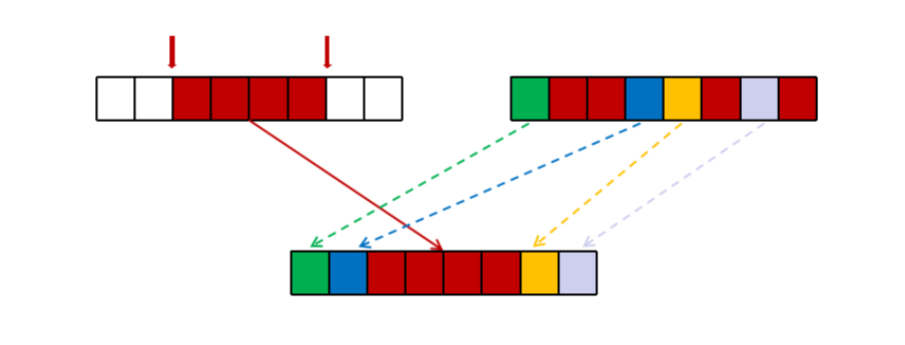
\includegraphics[width=3in]{crossover.png}
	\caption{crossover}
	\label{fig1}
	\end{figure}

\section{Experiments}

	In this project, I use python to implement the two algorithms. As for third party package, I only use `Numpy' (for math calculation) and `Matplotlib' (for plotting). Just execute `python tsp.py tsp/five\_d.txt' (the final arguments can be changed, any dataset that contains NxN distances can be solved by my script) to see the final result.

	Datasets are from `https://people.sc.fsu.edu/\~jburkardt/datasets/tsp/tsp.html'.

	The following table \ref{table1} listed the dataset together with given shortest tour distance and the solution I found.

	\begin{table}[htbp]
	\centering
	\caption{TSP solved by GA and SA}
	\label{table1}
	\begin{tabular}{|c|c|c|c|}
		\hline
		& & & \\[-3pt]
		dataset & gt        & SA        & GA \\\hline      & & & \\[-3pt]
		ATT48   & 33551 & 36077 & 39634 \\\hline & & & \\[-3pt]
DANTZIG42   & 699     & 733     & 950      \\\hline & & & \\[-3pt]
		FIVE      & 19        & 19        & 19        \\\hline & & & \\[-3pt]
		FRI26    & 937     & 953      & 1164    \\\hline & & & \\[-3pt]
		GR17     & 2085   & 2088   & 2153    \\\hline & & & \\[-3pt]
		P01        & 291     & 303      & 307    \\\hline
	\end{tabular}
	\end{table}

	The searching curve of SA and GA for each datasets are shown below:
	\newline
	\newline

	\begin{figure}[htbp]
	\centering
	\subfigure[ATT48-SA]{\begin{minipage}[t]{0.45\linewidth}
	\centering
	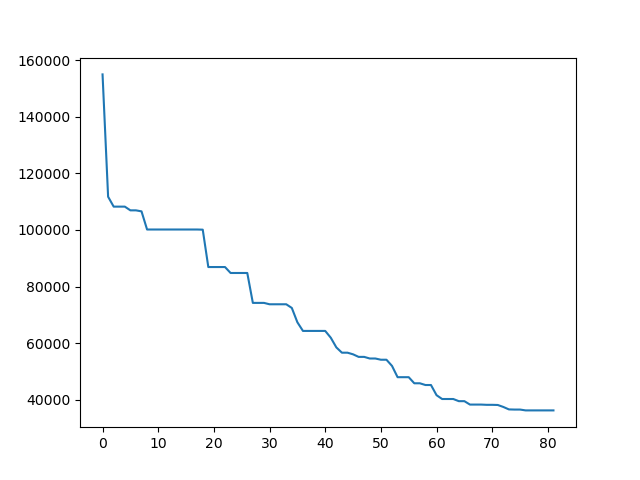
\includegraphics[width=\linewidth]{tsp/att48_d_sa.png}
	\end{minipage}
	}
	\subfigure[ATT48-GA]{\begin{minipage}[t]{0.45\linewidth}
	\centering
	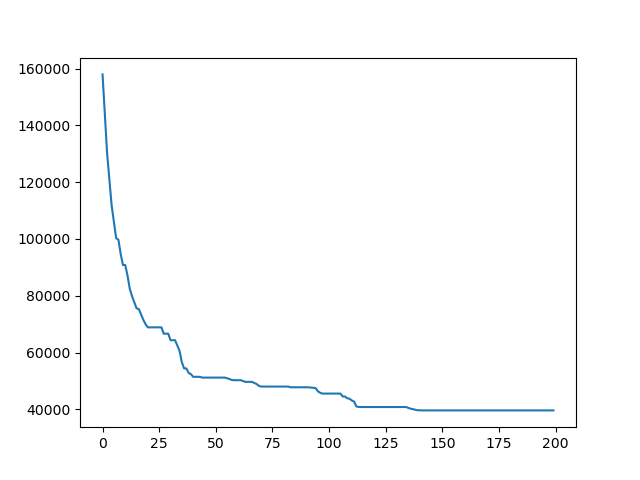
\includegraphics[width=\linewidth]{tsp/att48_d_ga.png}
	\end{minipage}
	}

	\subfigure[DANTZIG42-SA]{\begin{minipage}[t]{0.45\linewidth}
	\centering
	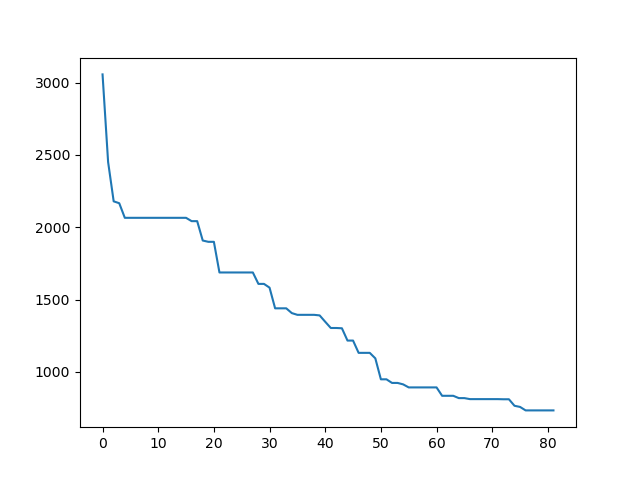
\includegraphics[width=\linewidth]{tsp/dantzig42_d_sa.png}
	\end{minipage}
	}
	\subfigure[DANTZIG42-GA]{\begin{minipage}[t]{0.45\linewidth}
	\centering
	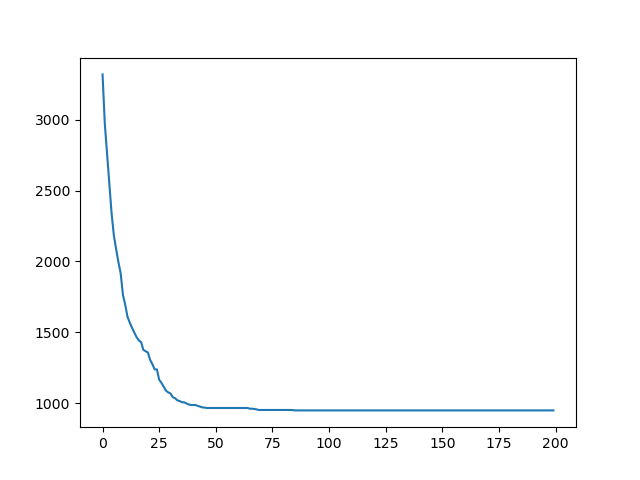
\includegraphics[width=\linewidth]{tsp/dantzig42_d_ga.png}
	\end{minipage}
	}

	\subfigure[FIVE-SA]{\begin{minipage}[t]{0.45\linewidth}
	\centering
	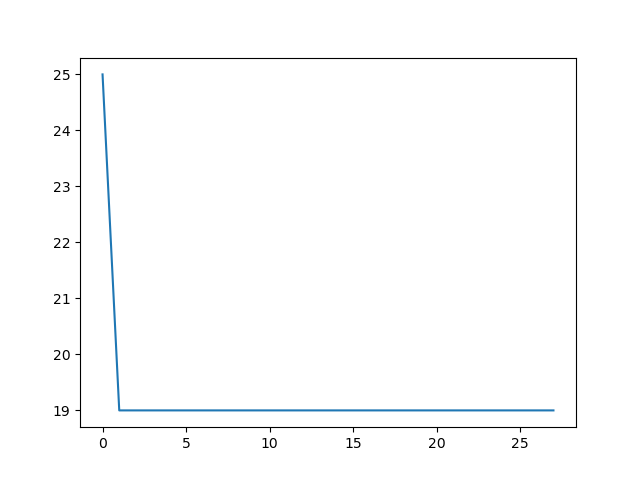
\includegraphics[width=\linewidth]{tsp/five_d_sa.png}
	\end{minipage}
	}
	\subfigure[FIVE-GA]{\begin{minipage}[t]{0.45\linewidth}
	\centering
	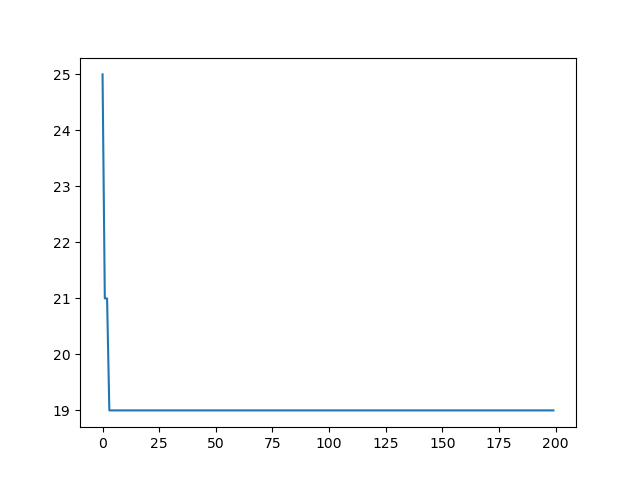
\includegraphics[width=\linewidth]{tsp/five_d_ga.png}
	\end{minipage}
	}

	\subfigure[FRI26-SA]{\begin{minipage}[t]{0.45\linewidth}
	\centering
	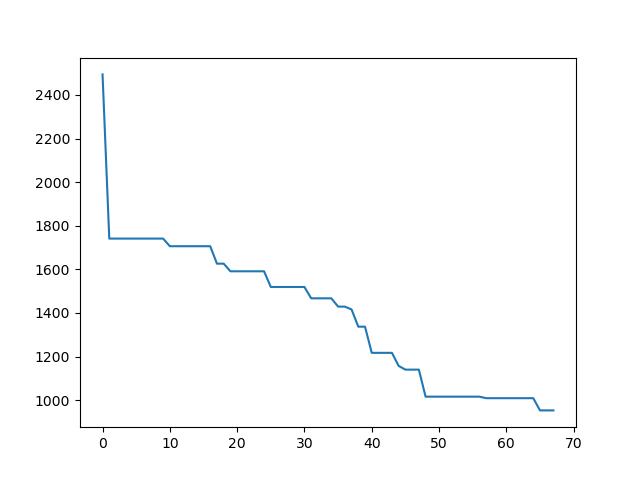
\includegraphics[width=\linewidth]{tsp/fri26_d_sa.png}
	\end{minipage}
	}
	\subfigure[FRI26-GA]{\begin{minipage}[t]{0.45\linewidth}
	\centering
	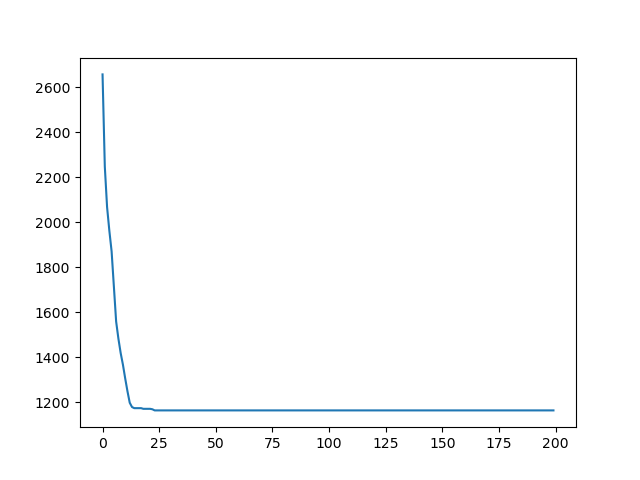
\includegraphics[width=\linewidth]{tsp/fri26_d_ga.png}
	\end{minipage}
	}
	\end{figure}
	\begin{figure}[!htbp]
	\centering
	\ContinuedFloat
	\subfigure[GR17-SA]{\begin{minipage}[t]{0.45\linewidth}
	\centering
	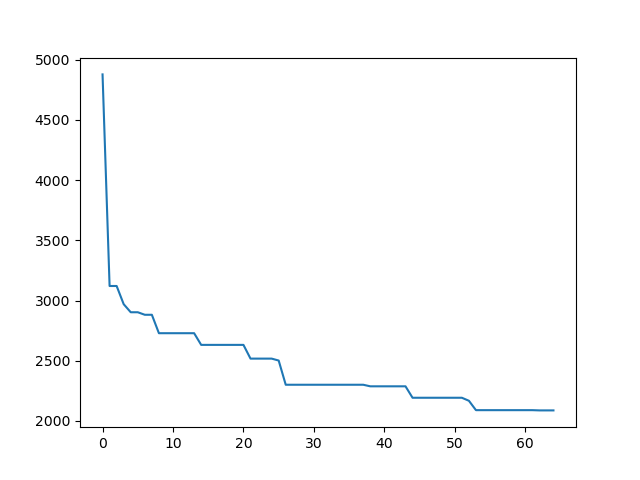
\includegraphics[width=\linewidth]{tsp/gr17_d_sa.png}
	\end{minipage}
	}
	\subfigure[GR17-GA]{\begin{minipage}[t]{0.45\linewidth}
	\centering
	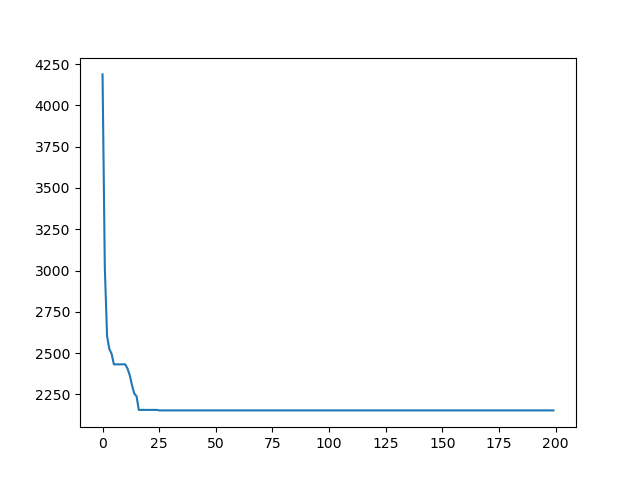
\includegraphics[width=\linewidth]{tsp/gr17_d_ga.png}
	\end{minipage}
	}

	\subfigure[P01-SA]{\begin{minipage}[t]{0.45\linewidth}
	\centering
	\includegraphics[width=\linewidth]{tsp/P01_d_sa.png}
	\end{minipage}
	}
	\subfigure[P01-GA]{\begin{minipage}[t]{0.45\linewidth}
	\centering
	\includegraphics[width=\linewidth]{tsp/P01_d_ga.png}
	\end{minipage}
	}
	\caption{Searching curves}
	\end{figure}

	According to the experimental result, we can see that 1) Both SA and GA can find satisfied solution, and SA seems to be better than GA; 2) my method to set the hyper-parameters enable a careful and efficient search of solution space, and can reach the satisfied solutions.

\begin{thebibliography}{99}
\bibitem{ref1} Van Buer M G, Woodruff D L, Olson R T. Solving the medium newspaper production/distribution problem[J]. European Journal of Operational Research, 1999, 115(2): 237-253.
\bibitem{ref2} Lawler E L ,  Lenstra J K ,  Kan A , et al. The Traveling Salesman Problem; A Guided Tour of Combinatorial Optimization[J]. Journal of the Operational Research Society, 1985, 37(5):535-536.
\bibitem{ref3} Kleywegt A J , Shapiro A . Stochastic Optimization. International Encyclopedia of the Social \& Behavioral Sciences, 2001.
\bibitem{ref4} Kirkpatrick S. Optimization by simulated annealing: Quantitative studies[J]. Journal of statistical physics, 1984, 34(5): 975-986.
\bibitem{ref5} Aarts E H L, Van Laarhoven P J M. Simulated annealing: an introduction[J]. Statistica Neerlandica, 1989, 43(1): 31-52.
\bibitem{ref6} Goldberg D E . Genetic Algorithm in Search, Optimization, and Machine Learning[M]. Addison-Wesley Pub. Co, 1989.
\bibitem{ref7} Sutton A, Neumann F. A parameterized runtime analysis of evolutionary algorithms for the Euclidean travelling salesperson problem[C]//Proceedings of the AAAI Conference on Artificial Intelligence. 2012, 26(1).
\bibitem{ref8} Kumar M, Husain M, Upreti N, et al. Genetic algorithm: Review and application[J]. International Journal of Information Technology, 2010, 2(2): 451-454.
\bibitem{ref9} Shukla A, Pandey H M, Mehrotra D. Comparative review of selection techniques in genetic algorithm[C]//2015 international conference on futuristic trends on computational analysis and knowledge management (ABLAZE). IEEE, 2015: 515-519.
\bibitem{ref10} Singh A, Baghel A S. A new grouping genetic algorithm approach to the multiple travelling salesperson problem[J]. Soft Computing, 2009, 13(1): 95-101.
\bibitem{ref11} Patil V P, Pawar D D. The optimal crossover or mutation rates in genetic algorithm: a review[J]. International Journal of Applied Engineering and Technology, 2015, 5(3): 38-41.
\end{thebibliography}

\end{document}
